%
\documentclass[12pt]{article}

% The usual packages
\usepackage{fullpage}
\usepackage{breakcites}
\usepackage{setspace}
\usepackage{endnotes}
\usepackage{float}
\usepackage{amsmath}
\usepackage{amsfonts}
\usepackage{amssymb}
\usepackage{rotating}
\usepackage{dcolumn}
\usepackage{longtable}
\usepackage{microtype}
\usepackage{graphicx}
\usepackage{hyperref}
%\usepackage[usenames,dvipsnames]{color}
\usepackage{url}
\usepackage{natbib}
\usepackage{framed}
\usepackage{epigraph}
\usepackage{lipsum}
\usepackage[font=small,labelfont=sc]{caption}
\restylefloat{table}
\bibpunct{(}{)}{;}{a}{}{,}

% Set paragraph spacing the way I like
\parskip=0pt
\parindent=20pt

% Define mathematical results
\newtheorem{lemma}{Lemma}
\newtheorem{proposition}{Proposition}
\newtheorem{theorem}{Theorem}
\newtheorem{claim}{Claim}
\newenvironment{proof}[1][Proof]{\begin{trivlist}
\item[\hskip \labelsep {\bfseries #1}]}{\end{trivlist}}
\newenvironment{definition}[1][Definition]{\begin{trivlist}
\item[\hskip \labelsep {\bfseries #1}]}{\end{trivlist}}
\newenvironment{example}[1][Example]{\begin{trivlist}
\item[\hskip \labelsep {\bfseries #1}]}{\end{trivlist}}
\newenvironment{remark}[1][Remark]{\begin{trivlist}
\item[\hskip \labelsep {\bfseries #1}]}{\end{trivlist}}

%% Set up fonts the way I like
%\usepackage{tgpagella}
%\usepackage[T1]{fontenc}
%\usepackage[bitstream-charter]{mathdesign}

%\usepackage{helvet}
\usepackage[labelfont={bf}, margin=0cm, font=small, skip=0pt]{caption}

% Baskervald
%\usepackage[lf]{Baskervaldx} % lining figures
%\usepackage[bigdelims,vvarbb]{newtxmath} % math italic letters from Nimbus Roman
%\usepackage[cal=boondoxo]{mathalfa} % mathcal from STIX, unslanted a bit
%\renewcommand*\oldstylenums[1]{\textosf{#1}}

\usepackage[T1]{fontenc}
\usepackage{newtxtext,newtxmath}


%% Set up lists the way I like
% Redefine the first level
\renewcommand{\theenumi}{\arabic{enumi}.}
\renewcommand{\labelenumi}{\theenumi}
% Redefine the second level
\renewcommand{\theenumii}{\alph{enumii}.}
\renewcommand{\labelenumii}{\theenumii}
% Redefine the third level
\renewcommand{\theenumiii}{\roman{enumiii}.}
\renewcommand{\labelenumiii}{\theenumiii}
% Redefine the fourth level
\renewcommand{\theenumiv}{\Alph{enumiv}.}
\renewcommand{\labelenumiv}{\theenumiv}
% Eliminate spacing around lists
\usepackage{enumitem}
\setlist{nolistsep}

% Create footnote command so that my name
% has an asterisk rather than a one.
\long\def\symbolfootnote[#1]#2{\begingroup%
\def\thefootnote{\fnsymbol{footnote}}\footnote[#1]{#2}\endgroup}

% Create the colors I want
\usepackage{color}
\definecolor{darkred}{RGB}{100,0,0}

\hypersetup{
 pdftitle={Logistic Regression with Small Samples}, % title
 pdfauthor={Kelly McCaskey and Carlisle Rainey}, % author
 pdfkeywords={logit}{probit}{logistic regression} {small sample} {bias}{bootstrap},
 pdfnewwindow=true, % links in new window
 colorlinks=true, % false: boxed links; true: colored links
 linkcolor=black, % color of internal links
 citecolor=black, % color of links to bibliography
 filecolor=black, % color of file links
 urlcolor=black % color of external links
}

% enable comments in pdf
\newcommand{\kelly}[1]{\textcolor{blue}{#1}}
\newcommand{\carlisle}[1]{\textcolor{magenta}{#1}}


\begin{document}

\begin{center}
{\LARGE Logistic Regression with Small Samples}\\\vspace{2mm}
{\large (Nearly) Unbiased Estimation with Penalized Maximum Likelihood\symbolfootnote[1]{We thank Alex Weisiger for making his data available to us. 
We thank Chris Zorn and participants at the 2015 Annual Meeting of the Society for Political Methodology for helpful comments.
We conducted these analyses analyses with \texttt{R} 3.1.0. 
All data and computer code necessary for replication are available at \href{https://www.github.com/kellymccaskey/small}{github.com/kellymccaskey/small}.}}\\\vspace{2mm}

\vspace{10mm}

Kelly McCaskey\symbolfootnote[2]{Kelly McCaskey is a Ph.D. student in the Department of Political Science, Texas A\&M University, 2010 Allen Building, College Station, TX, 77843 (\href{mailto:kellymccaskey@tamu.edu}{kellymccaskey@tamu.edu}).}

\vspace{3mm}

Carlisle Rainey\symbolfootnote[3]{Carlisle Rainey is Assistant Professor of Political Science, Texas A\&M University, 2010 Allen Building, College Station, TX, 77843 (\href{mailto:crainey@tamu.edu}{crainey@tamu.edu}).}
\end{center}

\vspace{10mm}

% Abstract
{\centerline{\textbf{Abstract}}}
\begin{quote}\noindent
In small samples, maximum likelihood estimates of logistic regression coefficients are substantially biased away from zero. 
This bias might be 25 percent or more in plausible scenarios. 
As a solution, we (re)introduce political scientists to Firth's (\citeyear{Firth1993}) penalty, which removes much of the bias from the usual estimator. 
We use Monte Carlo simulations to illustrate that penalized maximum likelihood estimation eliminates most of the bias, but also (perhaps more importantly) greatly reduces the variance of the estimate. 
We illustrate the substantive importance of the penalized estimator with replications of \cite{Weisiger2014} and \cite{GeorgeEpstein1992}.
 \end{quote}

% Remove page number from first page
\thispagestyle{empty}

% Start main text
\newpage
\onehalfspace

\section*{The Problem}

When modeling a binary outcome, the researcher might use logistic regression and model the probability of an event as $\text{Pr}(y_i) = \text{Pr}(y_i = 1~|~ X_i) = \dfrac{1}{1 + e^{-X_i\beta}}$, where $y$ represents a vector of binary outcomes, $X$ represents a matrix of explanatory variables and an intercept, and $\beta$ represents a vector of model coefficients. 
Using this model, it is straightforward to derive the likelihood function 
\begin{equation}\nonumber
\text{Pr}(y | \beta) = L(\beta | y) = \displaystyle \prod_{i = 1}^n \left[\left( \dfrac{1}{1 + e^{-X_i\beta}}\right)^{y_i}\left(1- \dfrac{1}{1 + e^{-X_i\beta}}\right)^{1 - y_i}\right]\text{.}
\end{equation}
\noindent As usual, one can take the natural logarithm of both sides to obtain the log-likelihood function 
\begin{equation}\nonumber
\log L(\beta | y) = \displaystyle \sum_{i = 1}^n \left[y_i \log \left( \dfrac{1}{1 + e^{-X_i\beta}}\right) + (1 - y_i) \log \left(1- \dfrac{1}{1 + e^{-X_i\beta}}\right)\right].
\end{equation}
\noindent The researcher can obtain the maximum likelihood (ML) estimate $\hat{\beta}^{mle}$ by finding the vector $\beta$ that maximizes $\log L$ \citep{King1989}. 

Asymptotically, the ML estimator for the logistic regression coefficient vector $\hat{\beta}^{mle}$ is centered at the true value $\beta^{true}$, so that $E(\hat{\beta}^{mle}) \approx \beta^{true}$ when the sample is large (\citealt{Wooldridge2002}, pp. 391-395, and \citealt{CasellaBerger2002}, p. 470).
For small samples, though, the asymptotic approximation does not work well--the ML estimates are biased substantially away from zero \citep[pp. 53-54]{Long1997}.
%The sampling distribution of $\hat{\beta}^{mle}$ is not centered at $\beta^{true}$, so that $E(\hat{\beta}^{mle}) \not\approx \beta^{true}$. 

Offering a rough heuristic about appropriate sample sizes, \cite[p. 54]{Long1997} writes: ``It is risky to use ML with samples smaller than 100, while samples larger than 500 seem adequate.''
This presents the researcher with a problem: When dealing with small samples, how can she obtain reasonable estimates of logistic regression coefficients?

\section*{A Solution}

The statistics literature offers a simple solution to the problem of bias. 
\cite{Firth1993} suggests penalizing the usual likelihood function $L(\beta | y)$ by a factor equal to the square root of the determinant of the information matrix $|I(\beta)|^\frac{1}{2}$, which produces a ``penalized'' likelihood function $L^*(\beta | y) = L(\beta | y)|I(\beta)|^\frac{1}{2}$ (see also \citealt{KosmidisFirth2009} and \citealt{Kosmidis2014}). 
It turns out that this penalty is equivalent to Jeffreys' (\citeyear{Jeffreys1946}) prior for the logistic regression model (\citealt{Firth1993} and \citealt{Poirier1994}).
Taking logs yields the penalized log-likelihood function.
\begin{equation}\nonumber
\log L^*(\beta | y) = \displaystyle \sum_{i = 1}^n \left[y_i \log \left( \dfrac{1}{1 + e^{-X_i\beta}}\right) + (1 - y_i) \log \left(1 - \dfrac{1}{1 + e^{-X_i\beta}}\right)\right] + \dfrac{1}{2} \log |I(\beta)|.
\end{equation}
Then the researcher can obtain the \emph{penalized} maximum likelihood (PML) estimate $\hat{\beta}^{pmle}$ by finding the vector $\beta$ that maximizes $\log L^*$. 
\cite{Zorn2005} suggested Firth's penalty for solving the problem of separation (see also \citealt{Rainey-separation}), but the broader application to small sample problems seems to have gone unnoticed in political science.

A researcher can implement PML just as easily as ML, but PML estimates of logistic regression coefficients are both less biased \citep{Firth1993} and more efficient \citep[p. 49]{Kosmidis2007} than ML estimates.\footnote{Further, the penalized maximum likelihood estimates are easy to calculate in R using the \texttt{logistf} or \texttt{brglm} packages. 
See the Section \ref{sec:pmle-in-R} of the Appendix for an example.}
This is important to note. 
When choosing between estimators, researchers often face a tradeoff between bias and efficiency \citep[pp. 37-38]{HastieTibshiraniFriedman2013}.
But there is no bias-variance tradeoff between ML and PML estimators.
The PML estimator exhibits both lower bias \textit{and} lower variance.

\section*{Simulations}

To demonstrate the substantial improvements in both bias and variance for small sample sizes sometimes found in political science research, we conduct a Monte Carlo simulation comparing the sampling distributions of the ML and PML estimates.
These simulations demonstrate two features of the ML and PML estimators:
\begin{enumerate}
\item The ML estimator can be quite biased in small samples, sometimes more than 50\%. The PML is nearly unbiased, regardless of sample size.
\item The variance of the ML estimator can be three or more times as large as the PML estimator.
\end{enumerate}
Of course, the increased bias and variance of the ML estimator means that the PML estimator will also have a much smaller mean squared error.

In our simulation, the true data generating process is always $\Pr(y_i = 1) = \frac{1}{1 + e^{-X_i \beta}}$, where $i \in 1, 2,..., n$ and $X_i \beta = \beta_{cons} + 0.5 x_1 + \sum_{j = 2}^k 0.2 x_j$. 
We consider the coefficient for $x_1$ as the coefficient of interest.
Each fixed $x_j$ is drawn from a normal distribution with mean of zero and standard deviation of one. 
The simulation varies the sample size $n$ from 30 to 210, the number of explanatory variables $k$ from 3 to 6 to 9, and the the intercept $\beta_{cons}$ from -1 to -0.5 to 0 (which, in turn, varies the proportion of events from about 28\% to 38\% to 50\%). 
We simulate 10,000 data sets for each combination of the simulation parameters and estimate the logistic regression coefficients using ML and PML for each data set.
We calculate mean and variance of each set of 10,000 coefficient estimates to estimate the mean and variance of the sampling distribution for each estimator. 

\subsection*{Bias}

We calculate the percent bias $= 100 \times \left(\frac{E(\hat{\beta})}{\beta^{true}} - 1 \right)$ as the sample size, the intercept (i.e., proportion of events), and number of explanatory variables vary.  
Figure \ref{fig:sims-coef-perc-bias} shows the results. 
The sample size varies across the x-axis of each plot and each panel shows a distinct combination of intercept and number of variables in the model. 
Across the range of the parameters of our sample, the bias of the MLE varies from about 120\% (intercept equal to -1, 9 predictors, and 30 observations) to around 2\% (intercept equal to zero, 3 predictors, and 210 observations). 
The bias in the PMLE, on the other hand, is much smaller. 
For the worst-case scenario with nine variables, 30 observations, and an intercept of -1 (about 11 events), the percent bias in the PMLE is only about seven percent.\footnote{Figures \ref{fig:ev} and \ref{fig:bias} in Section \ref{sec:app-sims} of the Appendix show the expected value and (absolute) bias of these estimates.}

\begin{figure}[h]
\begin{center}
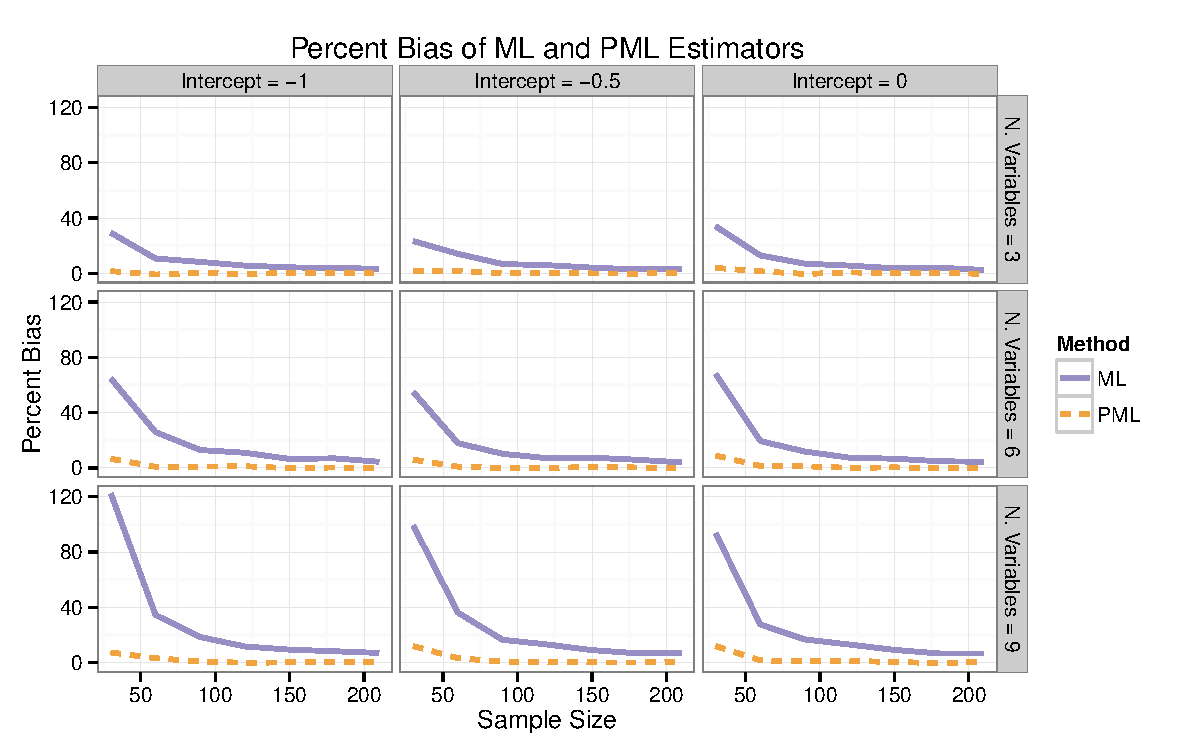
\includegraphics[width = \textwidth]{figs/sims-percent-bias.pdf}
\caption{This figure illustrates the substantial bias of $\hat{\beta}^{mle}$ and the near unbiasedness of $\hat{\beta}^{pmle}$.}\label{fig:sims-coef-perc-bias}
\end{center}
\end{figure}

\subsection*{Variance}

In many cases, estimators trade off bias and variance, but that is \textit{not} the case for ML and PML. 
Figure \ref{fig:sims-var} shows that, in addition to nearly eliminating the bias, PML also substantially reduces the variance of the estimator, especially for small sample sizes (less than about 75 observations in our simulations). 
For $N = 30$ and $\beta_{cons} = -1$ (about 28\% events), the variance of the ML estimator is about 95\%, 243\%, and 610\% larger than the PML estimator for 3, 6, and 9 variables, respectively. 
For $N = 60$, the variance is about 30\%, 58\% and 91\% larger, respectively. For a larger sample of $N = 210$, the variance is still about 7\%, 10\%, and 14\% larger for the ML estimator. 

The smaller variance is perhaps more important than the reduced bias.
Rather than focus on how close the averages of the estimates are to the true value (e.g., bias), a more important summary of estimator performance might be how far the estimates are from the true value, on average (e.g., mean squared error).
The mean squared error (MSE) equals $\frac{1}{n}\sum_{i=1}^n(\hat{\beta} - \beta^{true})^2 = \text{variance} + \text{bias}^2$.
The large differences in the variance and the relatively smaller differences in bias lead to substantial differences in the MSE of the two estimators.\footnote{Figures \ref{fig:var-infl}, \ref{fig:mse}, and \ref{fig:mse-infl} in Section \ref{sec:app-sims} of the Appendix show the variance inflation, mean squared error, and mean squared error inflation of the estimates.}

\begin{figure}[h]
\begin{center}
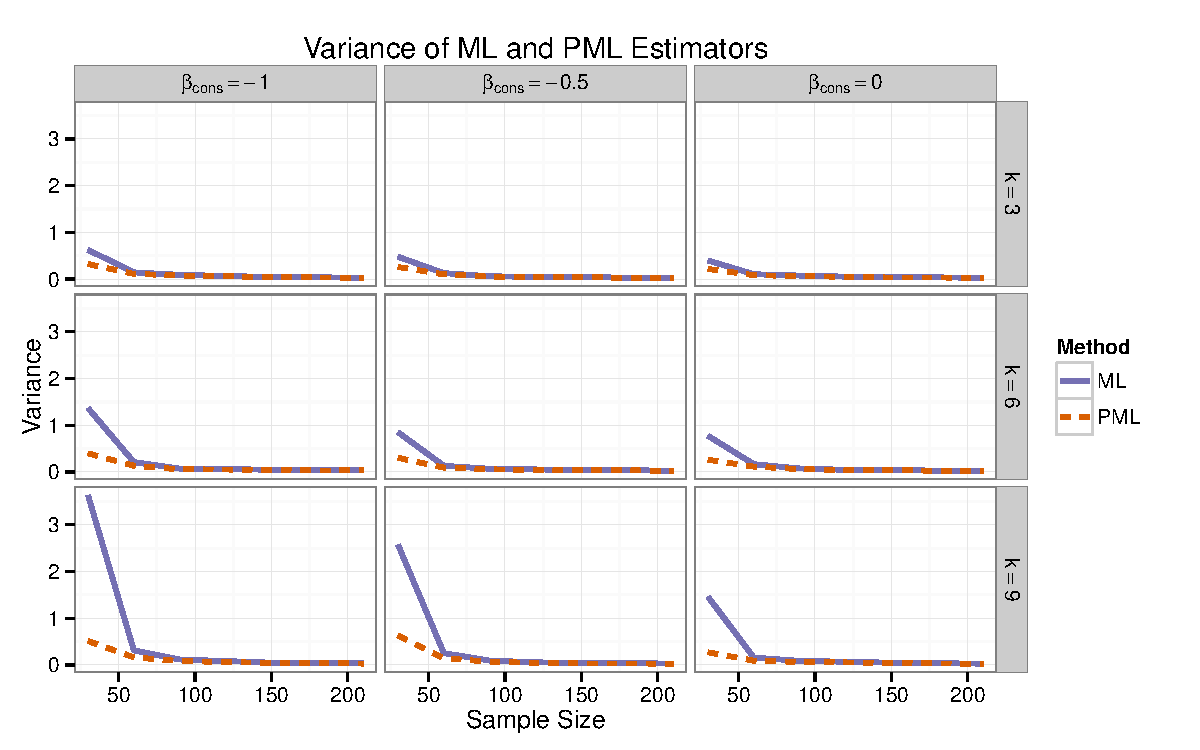
\includegraphics[width = \textwidth]{figs/sims-var.pdf}
\caption{This figure illustrates the smaller variance of $\hat{\beta}^{pmle}$ compared to $\hat{\beta}^{mle}$.}\label{fig:sims-var}
\end{center}
\end{figure}

These simulation results show that Firth's (1993) bias correction is not trivial. 
In small samples, ML estimates of logistic regression coefficients are severely biased.
The penalty identified by Firth nearly eliminates this bias, and, as a side effect, produces large gains in the efficiency of the estimates. 

%\section*{An Application}
\section*{Application}
\subsection*{Replication of \cite{Weisiger2014}}

To illustrate the potential importance of using the nearly unbiased PML estimator in an application, we reanalyze a portion of the statistical analysis in \cite{Weisiger2014}. 
Weisiger describes how, after the official end of the war, violence sometimes continues in the form of guerrilla warfare. 
He argues that resistance is more likely when conditions are favorable for insurgency, such as difficult terrain, a occupying force, or a pre-war leader remains at-large in the country. 

Weisiger's sample consists of 35 observations (with 14 insurgencies). 
We reanalyze Weisiger's data using logistic regression to show the substantial difference between the biased, high-variance ML estimates and the nearly unbiased, low-variance PML estimates. 
(Weisiger uses a linear probability model for in the original analysis, but that leads to probabilities that fall outside the $[0, 1]$ interval.)\footnote{Specifically, we reanalyze the Model 3 in Weisiger's Table 2 (p. 14). 
In the original analysis, Weisiger uses a linear probability model. 
He writes that ``I [Weisiger] make use of a linear probability model, which avoids problems with separation but introduces the possibility of non-meaningful predicted probabilities outside the [0,1] range'' (p. 11).
As he notes, predictions outside the $[0, 1]$ interval pose a problem for interpreting the linear probability model. 
In these data for example, the linear probability model estimates a probability of 1.41 of insurgency in one case. 
In another, it estimates a probability of -0.22. 
Overall, 25\% of the estimated probabilities based on the linear probability model are larger than one or less than zero.
Of course, these results are nonsense. 
However, because of the well-known small-sample bias, methodologists discourage researchers from using logistic regression with small samples.
The PML approach, though, solves the problem of bias as well as nonsense predictions.} Prior to estimation, we standardize the continuous variables to have mean zero and standard deviation one-half and binary variables to have mean zero \citep{Gelman2008}.
Figure \ref{fig:weisiger-coefs} shows the coefficient estimates and 90\% confidence intervals using ML and PML. 
Notice that the PML estimates are substantially smaller in many cases.
Although the coefficient for terrain only changes by 16\%, each of the remaining coefficients changes by more than 45\%! 
The coefficient for per capita GDP shrinks by more the 60\% and the coefficient for occupying force density grows by nearly 100\%.
Also notice that the PML standard errors are much smaller--the ML estimates for the coefficients of a coordinating leader and for the intercapital distance fall outside the PML 90\% confidence interval.
On average, the PML confidence intervals are about half as wide as the ML confidence intervals.

\begin{figure}[h]
\begin{center}
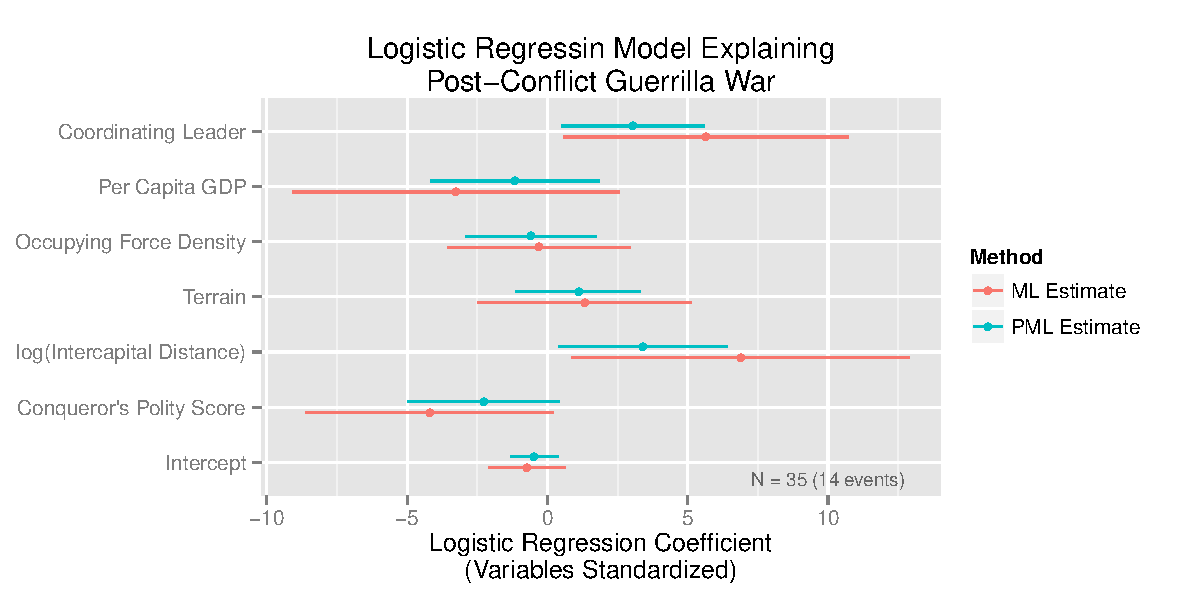
\includegraphics[width = \textwidth]{figs/weisiger-coefs.pdf}
\caption{This figure shows the coefficients for a logistic regression model estimated explaining post-conflict guerrilla war estimated with ML and PML. 
Notice that the PML estimates tend to be much smaller than the ML estimates.}\label{fig:weisiger-coefs}
\end{center}
\end{figure}

Because we do not know the true model, we cannot know which of these sets of coefficient is better. 
However, we can use out-of-sample prediction to help adjudicate between these two methods. 
We use leave-one-out cross-validation and summarize the prediction errors using Brier and log scores, for which smaller values indicate better predictive ability.\footnote{The Brier score is calculated as $\sum_{i = 1}^n (y_i - p_i)^2$, where $i$ indexes the observations, $y_i \in \{0, 1\}$ represents the actual outcome, and $p_i \in (0, 1)$ represents the estimated probability that $y_i = 1$. 
The log score as $-\sum_{i = 1}^n log(r_i)$, where $r_i = y_i p_i + (1 - y_i)(1 - p_i)$. 
Notice that because we are logging $r_i \in [0, 1]$, $\sum_{i = 1}^n log(r_i)$ is always negative and smaller (i.e., more negative) values indicate worse fit. 
We choose to take the negative of $\sum_{i = 1}^n log(r_i)$, so that, like the Brier score, larger values indicate a worse fit.} 
The ML estimates produce a Brier score of 0.14, and the PML estimates lower the Brier score by 14\% to 0.12. 
The ML estimates produce a log score of 0.58, while the PML estimates lower the log score by 34\% to 0.38. 
The PML estimates outperform the ML estimates for both approaches to scoring, and
this provides good evidence that the PML estimates better capture the data generating process.

Because we are using a logistic regression, we might be more interested in \textit{functions} of the coefficients than in the coefficients themselves. 
For an example, we focus on Weisiger's hypothesis that there will be a greater chance of resistance when the pre-conflict political leader remains at large in the conquered country.
Setting all other explanatory variables at their sample medians, we calculated the predicted probabilities, the first difference, and the risk ratio for the probability of a post-conflict guerrilla war as countries gain a coordinating leader. 
Figure \ref{fig:weisiger-qis} shows the estimates of the quantities of interest.

\begin{figure}[H]
\begin{center}
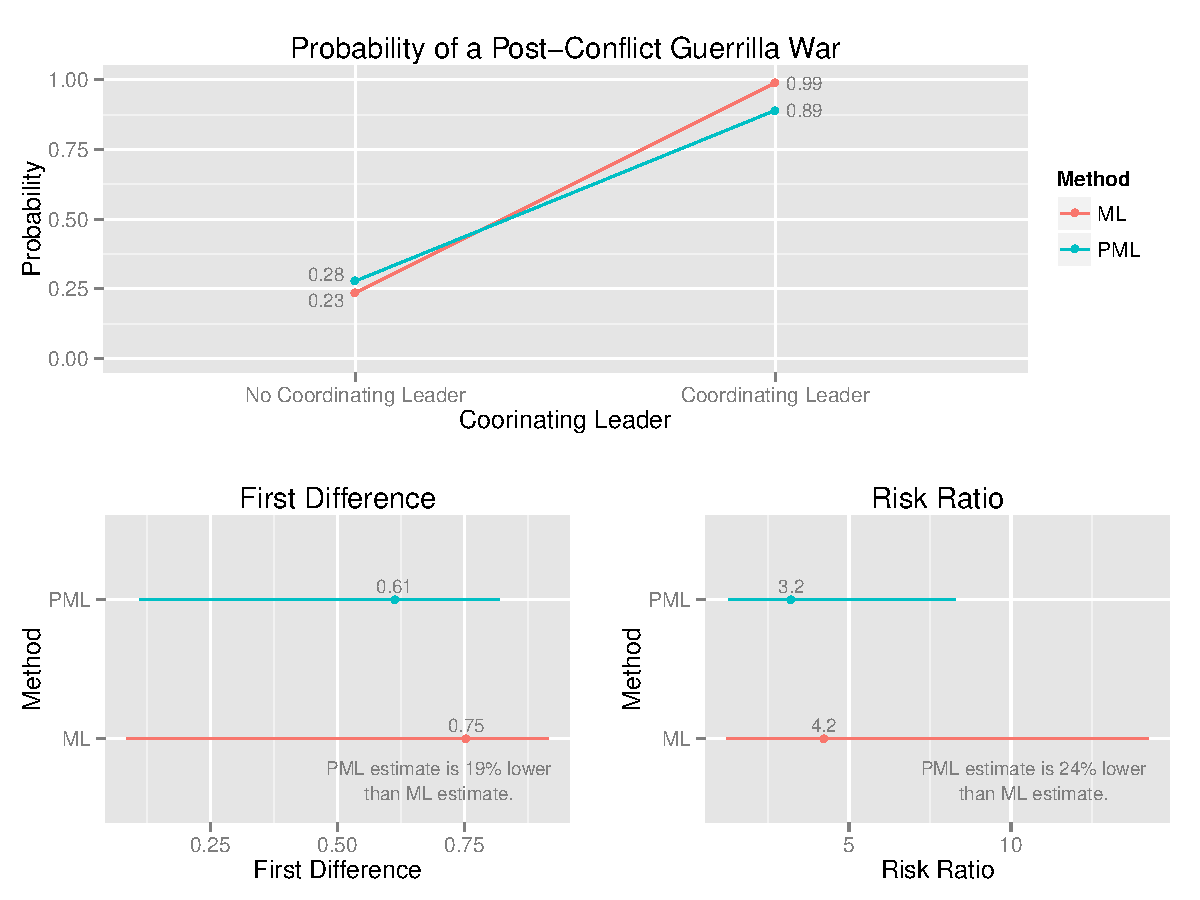
\includegraphics[width = \textwidth]{figs/weisiger-qis.pdf}
\caption{This figure shows the quantities of interest for the effect of a coordinating leader on the probability of a post-conflict guerrilla war.}\label{fig:weisiger-qis}
\end{center}
\end{figure}

PML pools the estimated probabilities toward zero, so that when a country lacks a coordinating leader, ML suggests a 23\% chance of rebellion while PML suggests a 28\% chance. 
On the other hand, when country \textit{does have} a coordinating leader, ML suggests a 99\% chance of rebellion of 0.99, but PML lowers this to 89\%. 
Accordingly, PML suggests smaller effect sizes, whether using a first difference or risk ratio. 
PML shrinks the estimated first difference by 19\% from 0.75 to 0.61 and the risk ratio by 24\% from 4.2 to 3.2.

\subsection*{Replication of \cite{GeorgeEpstein1992}}

In another application, we reanalyze the statistical analysis of the integrated model of U.S. Supreme Court decisions developed by \cite{GeorgeEpstein1992}. The authors combine the legal and extralegal models of  Court decision making in order to overcome the complementary idiosyncratic shortcomings of each. The legal model claims \emph{stare decisis}, or the rule of law, as the key determinant of future decisions while the extralegal model takes a behavioralist approach containing an array of sociological, psychological, and political factors. 

Like the previous example of the replication of \cite{Weisiger2014}, George and Epstein's sample consists of 64 Court decisions involving capital punishment from 1971 to 1988. They originally use maximum likelihood estimation so we reanalyze their data using both ML and PML to demonstrate the difference in the estimates with such a small sample. Figure \ref{fig:ge-coefs} illustrates the shift in coefficient estimates. In all cases, the PML estimate is smaller than the ML estimate. Each coefficient decreases by at least 25\% with three decreasing by more than 40\%: court change, the largest, at 49\%, solicitor general at 48\%, and political environment with 41\%. Additionally, the PML standard errors are all smaller than their ML counterparts. 

\begin{figure}[H]
\begin{center}
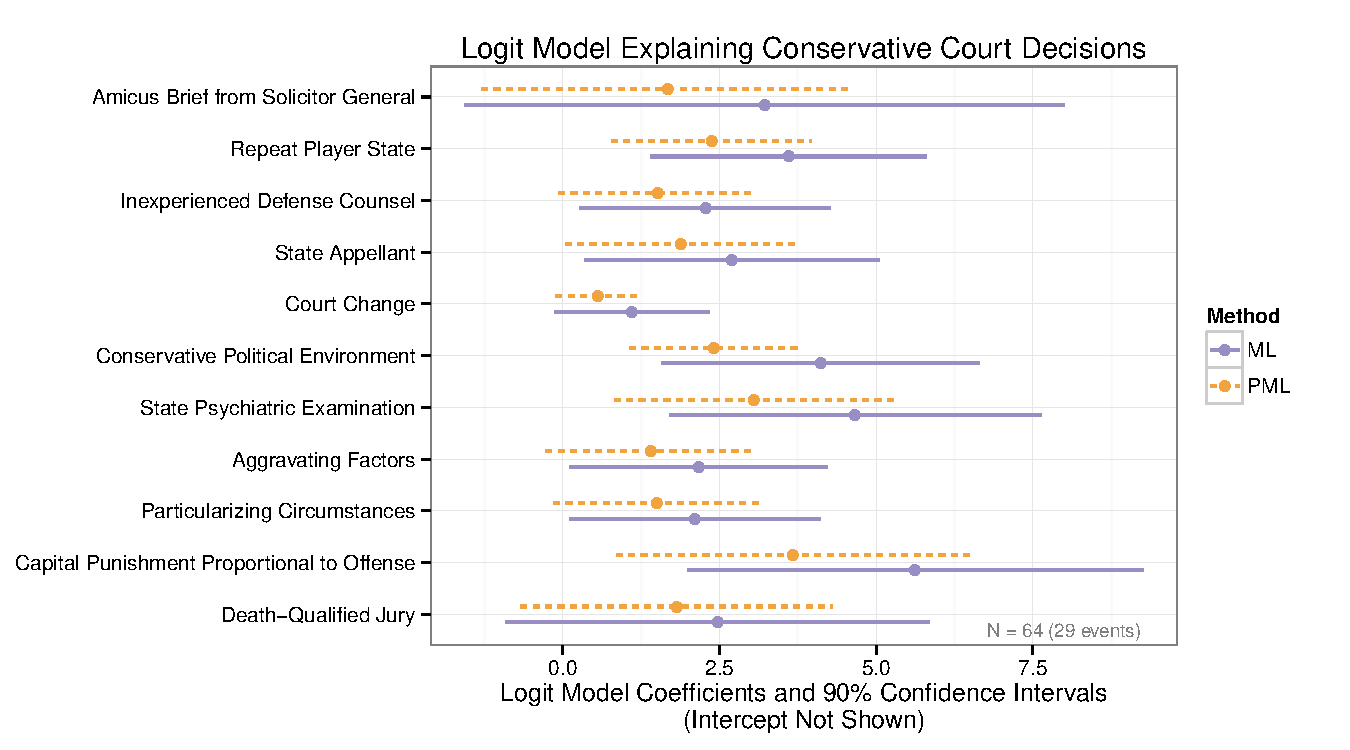
\includegraphics[width = \textwidth]{figs/ge-coefs.pdf}
\caption{This figure shows the coefficients for a logistic regression model estimating U.S. Supreme Court Decisions by both ML and PML. Note that the PML estimates are smaller with narrower variances than those of ML}\label{fig:ge-coefs}
\end{center}
\end{figure}

We use out-of-sample prediction to evaluate the performance of each model, as we are unable know the true model. Using leave-one-out cross-validation and summarizing the prediction errors with both Brier and log scores, we can be confident in our assertion that the PML process outperforms the ML. The ML estimates produce a Brier score of 0.17, and the PML estimates lower the Brier score by 8\% to 0.16. Similarly, the ML estimates produce a log score of 0.89, while the PML estimates lower the log score by 41\% to 0.53. 


\begin{figure}[H]
\begin{center}
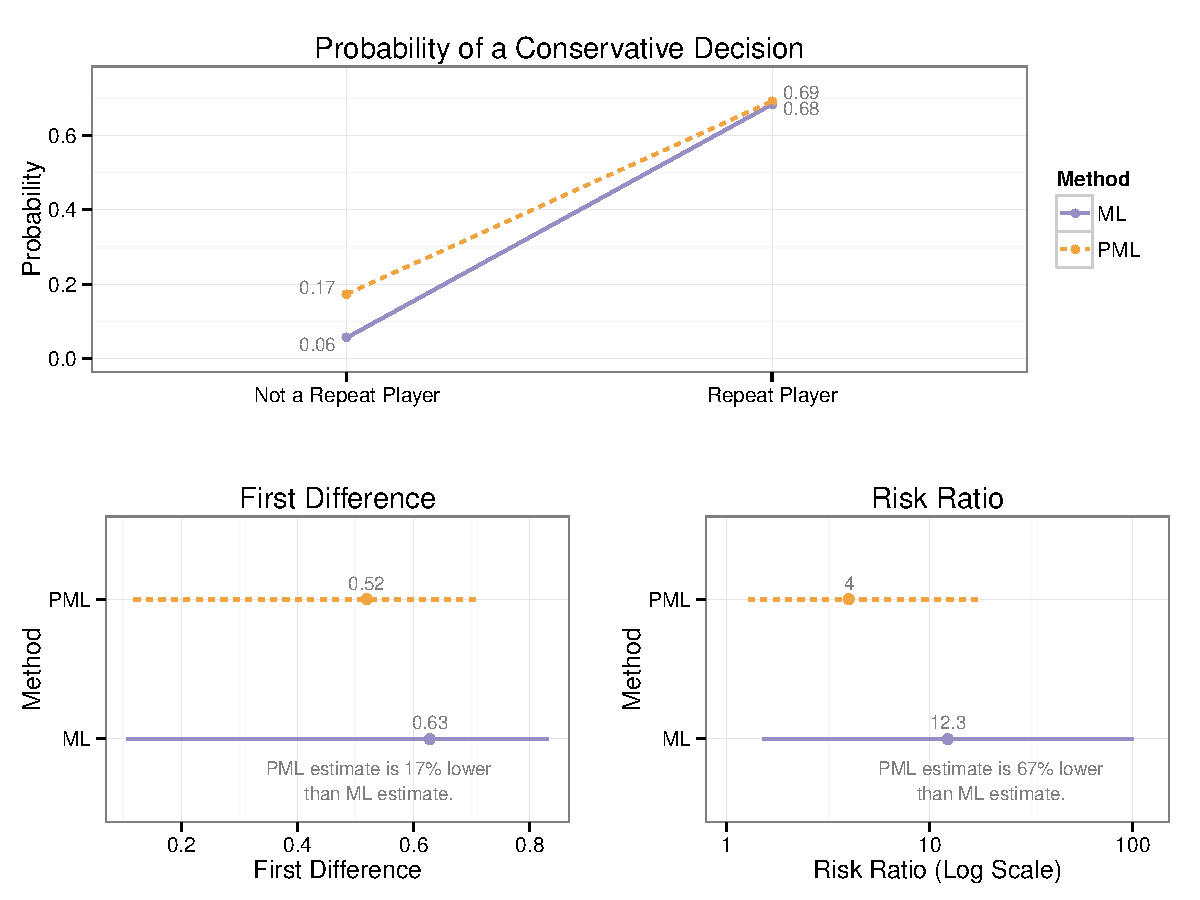
\includegraphics[width = \textwidth]{figs/ge-qis.pdf}
\caption{This figure shows the quantities of interest for the effect of the solicitor general filing a brief amicus curiae on the probability of a decision in favor of capital punishment.}\label{fig:ge-qis}
\end{center}
\end{figure}

Again, because we are using maximum likelihood, we are likely more interested in the functions of the coefficients rather than the coefficients themselves. For instance, we take George and Epstein's integrated model of Court decisions to determine the first difference and risk ratio for the probability of whether or not the Court decided in favor of capital punishment. We take whether or not the solicitor general filed an amicus curiae brief (coded as 1 if yes, 0 otherwise) and hold all other explanatory variables constant at their medians. Figure \ref{fig:ge-qis} shows the estimates of the quantities of interest.

As we know, PML pools the estimated probabilities toward, zero such that in the absence of an amicus curiae brief filed by the solicitor general, the PML estimates suggest 17\% chance of the Court deciding in favor of capital punishment while ML estimates a 6\% chance. When an amicus curiae brief was filed by the solicitor general, the Court has a 53\% chance of deciding in favor of capital punishment as compared to the 60\% chance suggested by ML. Thus, PML also provides smaller effect sizes, as well, for both the first difference and the risk ratio. PML decreases the estimated first difference by 35\% and the risk ratio by 75\%. 

\section*{Conclusion}

The substantial difference in these estimates demonstrates the potential importance of using PML when dealing with small samples and binary outcomes.
In small samples, ML leads to large biases in logistic regression coefficients. 
Further, these estimates are biased \textit{away} from zero, leading researchers to conclude that variables have larger effects than they actually do. 
However, PML is nearly unbiased, regardless of sample size. 
And these reductions in bias do not come at a large cost. 
Indeed, the PML estimates exhibit less bias, smaller variance, and lower mean squared error than the ML estimates.

\singlespace 
\newpage
\normalsize
\bibliographystyle{apsr_fs}
%\bibliography{/Users/carlislerainey/Dropbox/papers/bibliography/bibliography.bib}
\bibliography{/Users/kellymccaskey/Dropbox/projects/bibliography/bibliography.bib}

\newpage
\begin{appendix}
\begin{center}
{\LARGE Online Appendix}\\
\vspace{3mm}
{\large Logistic Regression in Small Samples}\\\vspace{2mm}
\end{center}

\section{Penalized Maximum Likelihood Estimation of Logistic Regression Models in R}\label{sec:pmle-in-R}

This example code is available at \href{https://github.com/kellymccaskey/small/blob/master/R/example.R}{https://github.com/kellymccaskey/small/blob/master/R/example.R}.

\begin{footnotesize}
\begin{verbatim}

# load data from web
library(readr)  # for read_csv()
weisiger <- read_csv("https://raw.githubusercontent.com/kellymccaskey/small/master/weisiger-replication/data/weisiger.csv") 

# quick look at data
library(dplyr)  # for glimpse()
glimpse(weisiger)

# model formula
f <- resist ~ polity_conq + lndist + terrain + 
  soldperterr + gdppc2 + coord

# ----------------------------- #
# pmle with the logistf package #
# ----------------------------- #

# estimate logistic regression with pmle
library(logistf)  # for logistf()
m1 <- logistf(f, data = weisiger)

# see coefficient estimates, confidence intervals, p-values, etc.
summary(m1)

# logistf does **NOT** work with texreg package
library(texreg)
screenreg(m1)

# see help file for more
help(logistf)

# --------------------------- #
# pmle with the brglm package #
# --------------------------- #

# estimate logistic regression with pmle
library(brglm)  # for brglm()
m2 <- brglm(f, family = binomial, data = weisiger)

# see coefficient estimates, standard errors, p-values, etc.
summary(m2)

# brglm works with texreg package
screenreg(m2)

# see help file for more
help(brglm)
\end{verbatim}
\end{footnotesize}



\section{Additional Simulation Results}\label{sec:app-sims}

\subsection{Expected Value}

\begin{figure}[H]
\begin{center}
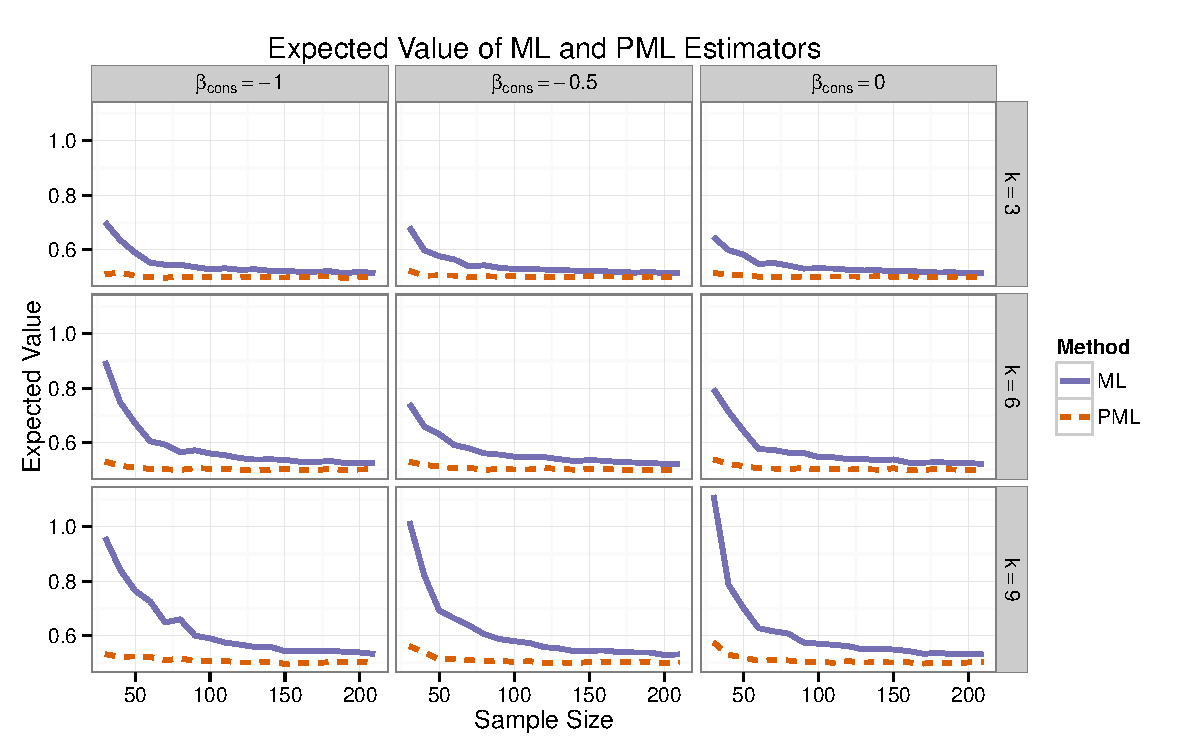
\includegraphics[width = \textwidth]{figs/sims-ev.pdf}
\caption{This figure shows the expected value of $\hat{\beta}^{mle}$ and $\hat{\beta}^{pmle}$. The true value is $\beta = 0.5$.}\label{fig:ev}
\end{center}
\end{figure}

\subsection{Bias}

\begin{figure}[H]
\begin{center}
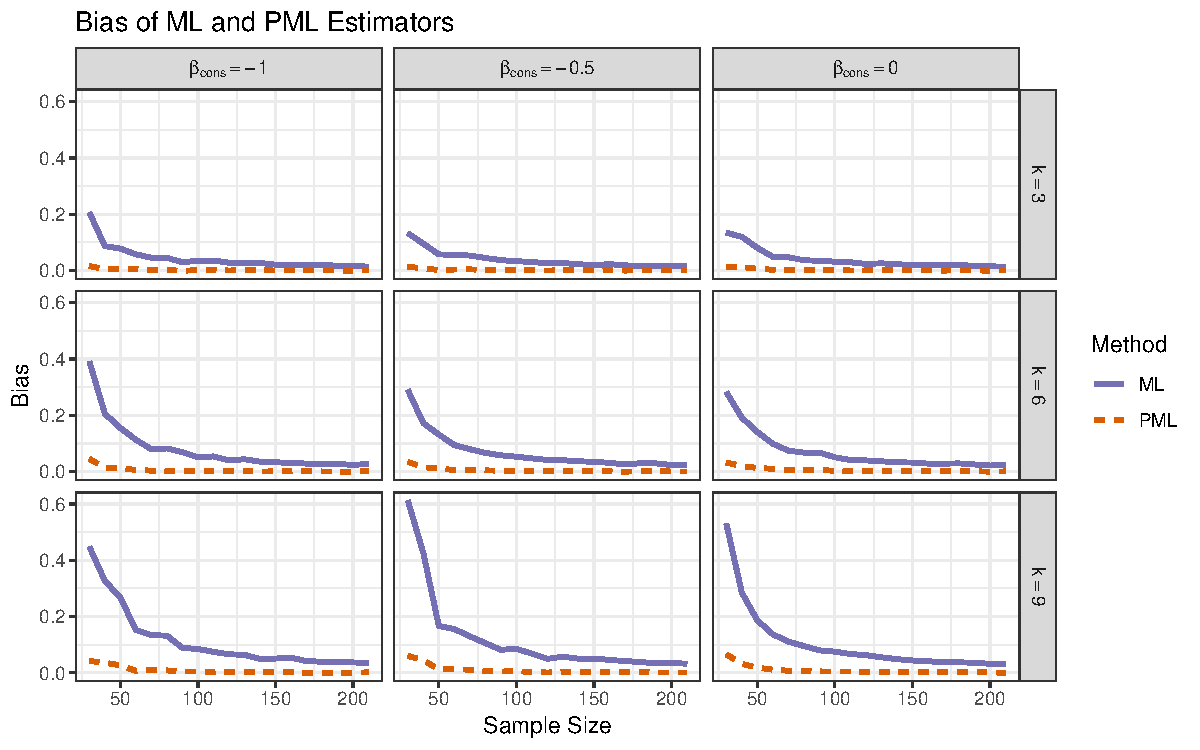
\includegraphics[width = \textwidth]{figs/sims-bias.pdf}
\caption{This figure shows the bias of $\hat{\beta}^{mle}$ and $\hat{\beta}^{pmle}$.}\label{fig:bias}
\end{center}
\end{figure}

\subsection{Variance Inflation}

\begin{figure}[H]
\begin{center}
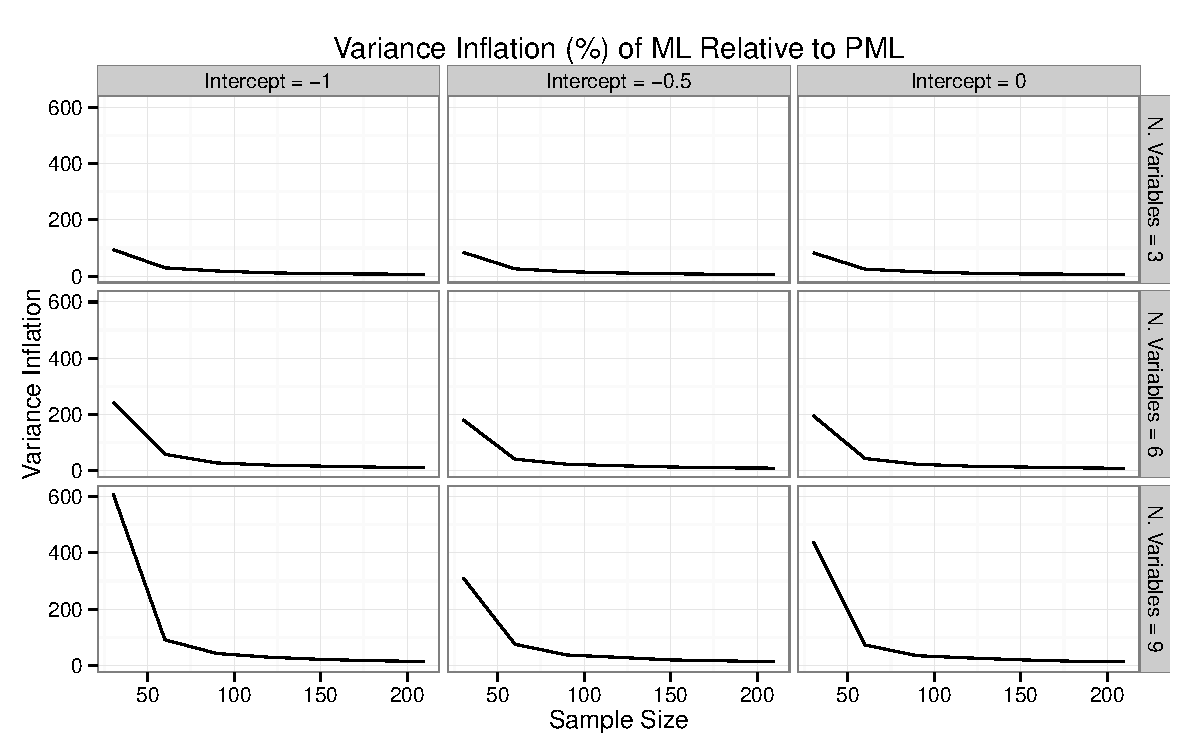
\includegraphics[width = \textwidth]{figs/sims-var-infl.pdf}
\caption{This figure shows the percent inflation in the variance of $\hat{\beta}^{mle}$ compared to $\hat{\beta}^{pmle}$.}\label{fig:var-infl}
\end{center}
\end{figure}

\subsection{Mean Squared Error}

\begin{figure}[H]
\begin{center}
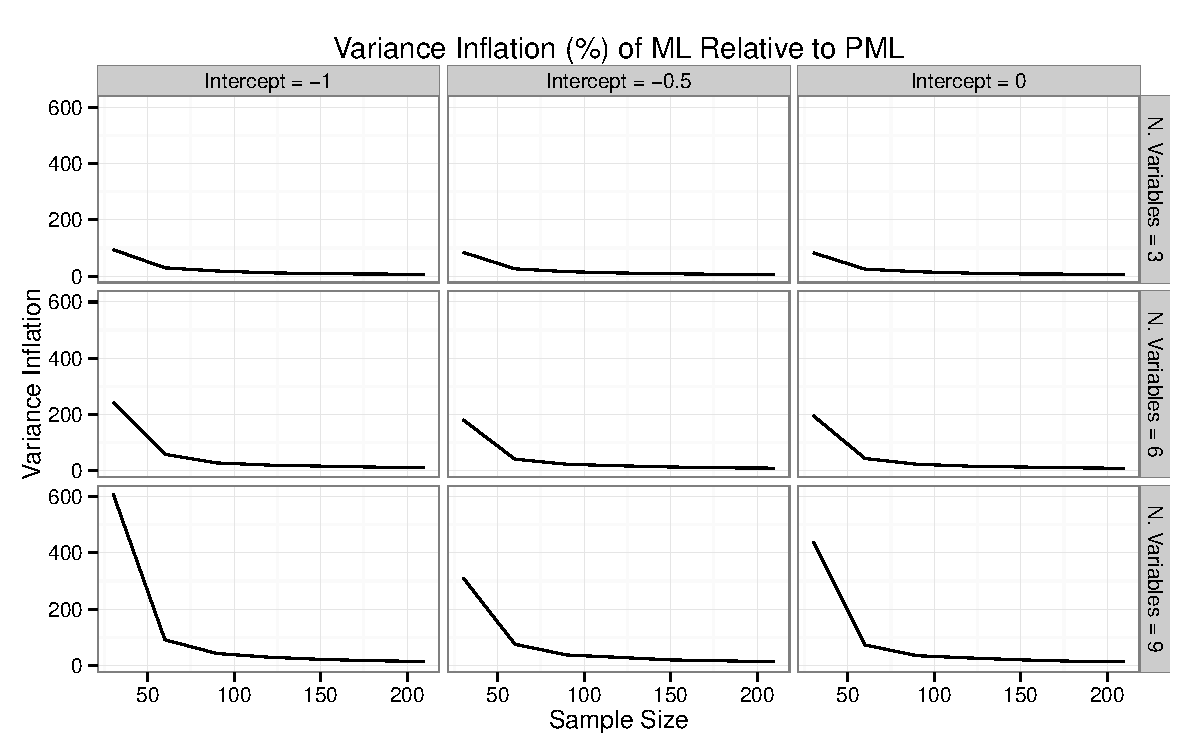
\includegraphics[width = \textwidth]{figs/sims-var-infl.pdf}
\caption{This figure shows the mean squared error of $\hat{\beta}^{mle}$ and $\hat{\beta}^{pmle}$.}\label{fig:mse}
\end{center}
\end{figure}

\subsection{Mean Squared Error Inflation}

\begin{figure}[H]
\begin{center}
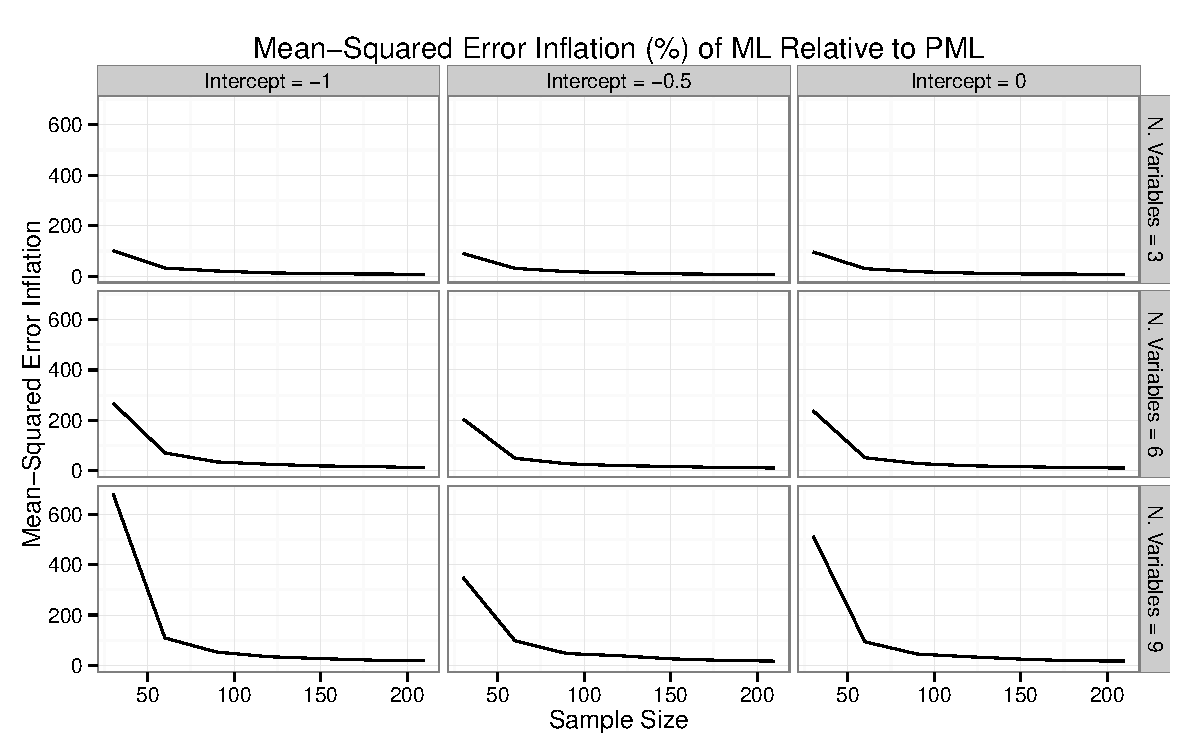
\includegraphics[width = \textwidth]{figs/sims-mse-infl.pdf}
\caption{This figure shows the percent increase in the mean square error of $\hat{\beta}^{mle}$ compared to $\hat{\beta}^{pmle}$.}\label{fig:mse-infl}
\end{center}
\end{figure}


\end{appendix}


\end{document}